\documentclass{article}
\usepackage{amsmath, amssymb,amsfonts,tikz}
\usetikzlibrary{shapes,arrows,calc,positioning,backgrounds}
\title{Algorithms \& Complexity: Lecture 1}
\author{Sam Barrett}
\newcommand{\qs}{q_{\texttt{start}}}
\newcommand{\qh}{q_{\texttt{halt}}}


\begin{document}

\maketitle

\section{Defining the Turing machine model}
\label{sec:definition}

In order to talk about the time taken or the space used by an algorithm, we require a precise \textbf{model of computation}. There are many proposed models, we will focus on the Turing machine as defined by Arora and Barak in their book.

\subsection{Arora-Barak Turing machines}

\subsubsection{Tapes}

A Turing machine is defined as having $k$ tapes where $k \geq 2$

\begin{itemize}
  \item The first tape is the \textit{input tape} and is \textbf{read-only}
  \item The $2..k-1$ tapes are \textit{work } tapes and are \textbf{read-write}
  \item The $k^{th}$ tape is the \textit{output} tape.
\end{itemize}

Each tape has a leftmost cell and \textit{potentially} infinitely many cells to the right of it. Potentially infinite meaning that at any given time, there are a finite number of cells but we can infinitely extend the tape over time.

Each tape has a \textbf{head} that sits on a cell and can move left and right.

\subsubsection{Alphabet}

A Turing machine also has an alphabet, denoted $\Gamma $. This is a \textbf{finite} set and it's elements are called \textit{symbols}. There are 4 primary symbols: $\rhd, \Box, 0, 1 $.

Here:

\begin{itemize}
  \item $\{ 0,1 \}^{*} $ is the set of bitstrings, the empty string is denoted with $\varepsilon$.
  \item $\rhd$ is the left-of-tape symbol and $\Box$ is the blank symbol
\end{itemize}

At any point in time, each cell of each tape contains a symbol. All but a finite number will be blank ($\Box$)

\subsubsection{Inital configuration}

The input tape has $\rhd$ on the leftmost cell, then a bitstring (the \textbf{input}) and the rest of the tape is blank. The work tapes (including the output tape) have $\rhd$ on the leftmost cell and the rest are blank.
Each tape starts with it's head on it's the leftmost cell.

\subsubsection{Computation step}

In a single step of computation the machine:

\begin{itemize}
  \item reads the character at each tape head
  \item writes a character at each work tape head
  \item may move each tape head to the left or to the right. \textbf{note: our tapes are not recursive, if a head on the leftmost cell moves left, it stays put}
\end{itemize}

\subsubsection{Formal definition}

A \textbf{Turing machine} is defined as a (6) tuple, $M = (k, \Gamma, Q, q_{\texttt{start}}, q_{\texttt{halt} },\delta )$ consists of the following data:

\begin{itemize}
  \item the number of tapes, $k$, $k \geq 2$
  \item the alphabet $\{ 0,1,\rhd,\Box \} \subseteq \Gamma $
  \item a finite set of $Q$ states, including the start state $q_{\texttt{start} }$ and the halt state $q_{\texttt{halt} }$
  \item a transition function, $\delta: Q \times \Gamma^{k} \rightarrow Q \times \Gamma^{k-1}\times \{ L,R,S \}^{k} $
        Where:
        \begin{itemize}
          \item the initial $Q$ is the state at the start of transition
          \item $\Gamma^{k}$ is the set of symbols read
          \item the final $Q$ is the state at the end of transition
          \item $\Gamma^{k-1}$ is the set of symbols written
          \item $\{ L,R,S \}^{k} $ is the set of movement instructions where:
                \begin{itemize}
                  \item $L$ means \textit{move left}
                  \item $R$ means \textit{move right}
                  \item $S$ means \textit{stay}
                \end{itemize}
        \end{itemize}

        \textbf{Note: we read $k$ symbols but only write $k-1$ symbols as we do not write on the input tape, we also have $k$ movement instructions as we are able to move on all $k$ of the tapes.}
\end{itemize}

\subsubsection{Example transition}

Say we have $k=$, and $\Gamma = \{ \rhd, \Box, 0 ,1 \} $ and $Q = \{ 4,5,6,7,8 \} $ with $q_{\texttt{start} } = 4$ and $q_{\texttt{halt} } = 8$.
We are currently in state 7 and the three tapes respectively say 1 (input), 1 (work) and $\Box$ (output).

Say that $\delta(7, \langle 1,1 \Box \rangle ) = (5, \langle 0, \Box \rangle , \langle L,L,S \rangle )$ then we:

\begin{itemize}
  \item transition to state 5
  \item overwrite thje 1 on the work tape with 0
  \item overwrite the $\Box$ on the output tape with $\Box$ (no change)
  \item move left on the input tape (if possible)
  \item move left on the work tape (if possible)
        \item stay put on the output tape
\end{itemize}

\textbf{We do not transition from the halt state (regardless of $\delta$)}

\section{Computing with Turing machines}

\subsection{Computing a function}

Given a function $f : \{ 0,1 \} ^{*} \rightarrow \{ 0,1 \} ^{* }$ a Turing machine $M = (k, \Gamma, Q, q_{\texttt{start}}, q_{\texttt{halt} }, \delta)$,

\begin{enumerate}
  \item what does it mean to say that $M$ \textbf{computes} $f$?

        It means that for every bitstring $x \in \{ 0,1 \}^{*}$, if we start in state $\qs$ with the initial configuration showing $x$ (meaning $x$ appears on the input tape and and the work tapes are blank), when we run $M$, we eventually reach $\qh$ with the output tape showing $\rhd$ on the leftmost cell and then the bitstring $f(x)$ followed by all blanks.
\end{enumerate}

Our initial configuration can be shown as:

\begin{center}
  \textbf{Input tape:}
  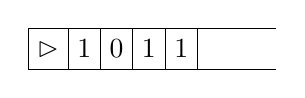
\begin{tikzpicture}[every node/.style={block},
  block/.style={minimum height=1.5em,outer sep=0pt,draw,rectangle,node distance=0pt}]


        \node (A) {$\rhd$};
        \node (B) [right = of A] {1};
        \node (C) [right = of B] {0};
        \node (D) [right = of C] {1};
        \node (E) [right = of D] {1};

        \draw (E.north east) -- ++(1cm,0) (E.south east) -- ++ (1cm,0);
               \end{tikzpicture}

\textbf{Work tapes:}
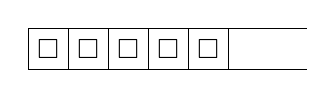
\begin{tikzpicture}[every node/.style={block},
        block/.style={minimum height=1.5em,minimum width=1em, outer sep=0pt,draw,rectangle,node distance=0pt}]

        \node (A) {$\Box$};
        \node (B) [right = of A] {$\Box$};
        \node (C) [right = of B] {$\Box$};
        \node (D) [right = of C] {$\Box$};
        \node (E) [right = of D] {$\Box$};

        \draw (E.north east) -- ++(1cm,0) (E.south east) -- ++ (1cm,0);
               \end{tikzpicture}

\textbf{Output tape: (also a work tape)}
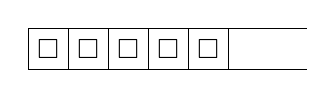
\begin{tikzpicture}[every node/.style={block},
        block/.style={minimum height=1.5em,minimum width=1em,outer sep=0pt,draw,rectangle,node distance=0pt}]

        \node (a) {$\Box$};
        \node (b) [right = of a] {$\Box$};
        \node (c) [right = of b] {$\Box$};
        \node (d) [right = of c] {$\Box$};
        \node (e) [right = of d] {$\Box$};

        \draw (e.north east) -- ++(1cm,0) (e.south east) -- ++ (1cm,0);
\end{tikzpicture}
\end{center}


Given that $f(x) = 0110111$, our required output tape will then be as follows:

\begin{center}
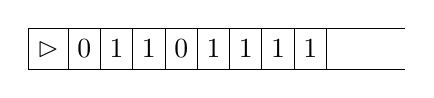
\begin{tikzpicture}[every node/.style={block},
        block/.style={minimum height=1.5em,minimum width=1em,outer sep=0pt,draw,rectangle,node distance=0pt}]

        \node (a) {$\rhd$};
        \node (b) [right = of a] {0};
        \node (c) [right = of b] {1};
        \node (d) [right = of c] {1};
        \node (e) [right = of d] {0};
        \node (f) [right = of e] {1};
        \node (g) [right = of f] {1};
        \node (h) [right = of g] {1};
        \node (i) [right = of h] {1};

        \draw (i.north east) -- ++(1cm,0) (i.south east) -- ++ (1cm,0);
\end{tikzpicture}
\end{center}

If the machine, $M$ does \textit{this} for every bitstring $x$ then we say it \textbf{computes} $f$. In the Arora-Barak definition, it does not matter what is on the work tape at the end of execution or the location of the work heads.

\subsection{Computable functions}

We say a function $f : \{ 0,1 \} ^{*} \rightarrow \{ 0,1 \} ^{*}$ or a function $f$ from bitstrings to bitstrings is \textbf{computable} if there exists some Turing machine that computes it and \textbf{non-computable} if there isn't.

In the second case where there exists no Turing machine that computes a function, is there some other kind of machine that \textit{does} compute it?

\subsubsection{Church's thesis}

We have only looked at one definition of Turing machines, there are many different variations that have been studied. 1 tape vs $\infty$ tapes, large alphabets, tapes infinite in both directions, 2D tapes, etc.

\textbf{None} of these variations affect our definition of computability. The same definition holds for all models that have been investigated, leading to Church's thesis which (informally) states:


\tikzstyle{background rectangle}=[thin,draw=black]
\begin{center}
  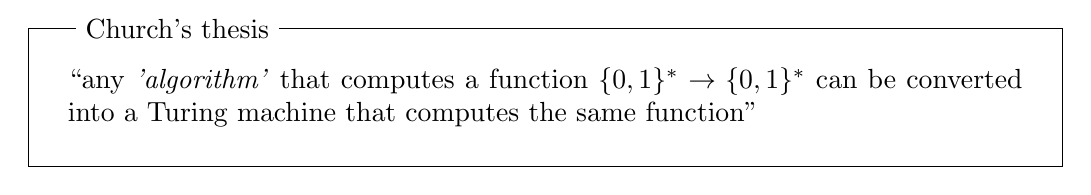
\begin{tikzpicture}[show background rectangle]
    \node[align=justify, text width=\textwidth, inner sep=1em]{
      ``any \textit{'algorithm'} that computes a function $\{ 0,1 \} ^{*} \rightarrow \{ 0,1 \} ^{*}$ can be converted into a Turing machine that computes the same function''
  };

  \node[xshift=3ex, yshift=-0.7ex, overlay, fill=white, draw=white, above
  right] at (current bounding box.north west) {
    Church's thesis
  };
  \end{tikzpicture}
\end{center}

\subsection{Boolean functions and language}

A language can be defined as any set of \textit{words}, for example \textit{all the words with an even occurrence of 1} is a language.


A \textbf{boolean function} is a function of the form: $f : \{ 0,1 \}^{*} \rightarrow \{ 0,1 \} $. Noting that the output is a single bit rather than a bitstring.

A important point about languages and boolean function is that they correspond. There is a one-to-one correspondence in fact between languages and boolean functions.
\begin{itemize}
  \item For a given boolean function $f$ the corresponding language is the set of bitstrings $x$ s.t. $f(x) = 1$
  \item For a language $L$, the corresponding boolean function sends $x$ to 1 if $x \in L$ and to $0$ otherwise.
\end{itemize}

This allows us to treat boolean functions, languages and decision problems as essentially the same thing.

A decision problem is said to be \textbf{deciadable} when the corresponding boolean function is \textbf{computable}. I.e. given a language $L$, for $L$ to be decidable there must exist some Turing machine that will start with a bitstring $x$ and will run continuously until it halts and upon halting there will be a $1$ on the output tape if $x \in L$ or $0$ if it is not in the language.

\subsubsection{Example: palindromes}

A \textbf{palindrome} is a bitstring that \textit{reads} the same forwards as backwards.

We can define our decision procedure for $\texttt{PAL} $, the set of all palindromes as:

\begin{enumerate}
  \item Copy the input to the work tape
  \item Move the input head to the start of the input
  \item move the input head to the right while moving the output head to the left. If at any moment, the machine observes two different values, it writes 0 to the output tape and halts
  \item Write 1 to the output tape and halt
\end{enumerate}

We can represent this as a Turing machine with 3 tapes and 5 states in the following example:

\underline{Step 1:}

\textbf{Input tape:}
\begin{center}

  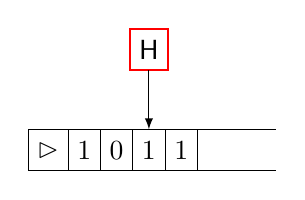
\begin{tikzpicture}[every node/.style={block},
  block/.style={minimum height=1.5em,outer sep=0pt,draw,rectangle,node distance=0pt}]


        \node (A) {$\rhd$};
        \node (B) [right = of A] {1};
        \node (C) [right = of B] {0};
        \node (D) [right = of C] {1};
        \node (E) [right = of D] {1};

        \node (F) [above = 0.75cm of D,draw=red,thick] {\textsf H};
        \draw[-latex] (F) -- (D);

        \draw (E.north east) -- ++(1cm,0) (E.south east) -- ++ (1cm,0);
      \end{tikzpicture}

\end{center}

\textbf{Work tape:}
\begin{center}

  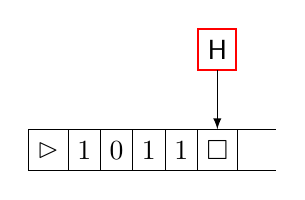
\begin{tikzpicture}[every node/.style={block},
  block/.style={minimum height=1.5em,outer sep=0pt,draw,rectangle,node distance=0pt}]

        \node (A) {$\rhd$};
        \node (B) [right = of A] {1};
        \node (C) [right = of B] {0};
        \node (D) [right = of C] {1};
        \node (E) [right = of D] {1};
        \node (G) [right = of E] {$\Box$};

        \node (F) [above = 0.75cm of G,draw=red,thick] {\textsf H};
        \draw[-latex] (F) -- (G);

        \draw (E.north east) -- ++(1cm,0) (E.south east) -- ++ (1cm,0);
      \end{tikzpicture}

\end{center}

\textbf{Output tape:}
\begin{center}

  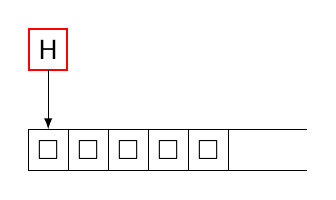
\begin{tikzpicture}[every node/.style={block},
  block/.style={minimum height=1.5em,outer sep=0pt,draw,rectangle,node distance=0pt}]


        \node (A) {$\Box$};
        \node (B) [right = of A] {$\Box$};
        \node (C) [right = of B] {$\Box$};
        \node (D) [right = of C] {$\Box$};
        \node (E) [right = of D] {$\Box$};

        \node (F) [above = 0.75cm of A,draw=red,thick] {\textsf H};
        \draw[-latex] (F) -- (A);

        \draw (E.north east) -- ++(1cm,0) (E.south east) -- ++ (1cm,0);
      \end{tikzpicture}

\end{center}

\underline{Step 2:}

\textbf{Input tape:}
\begin{center}

  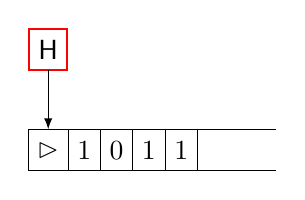
\begin{tikzpicture}[every node/.style={block},
  block/.style={minimum height=1.5em,outer sep=0pt,draw,rectangle,node distance=0pt}]


        \node (A) {$\rhd$};
        \node (B) [right = of A] {1};
        \node (C) [right = of B] {0};
        \node (D) [right = of C] {1};
        \node (E) [right = of D] {1};

        \node (F) [above = 0.75cm of A,draw=red,thick] {\textsf H};
        \draw[-latex] (F) -- (A);

        \draw (E.north east) -- ++(1cm,0) (E.south east) -- ++ (1cm,0);
      \end{tikzpicture}

\end{center}

\textbf{Work tape:}
\begin{center}

  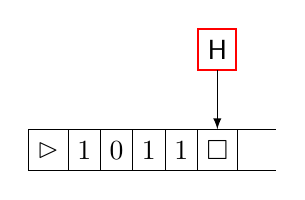
\begin{tikzpicture}[every node/.style={block},
  block/.style={minimum height=1.5em,outer sep=0pt,draw,rectangle,node distance=0pt}]



        \node (A) {$\rhd$};
        \node (B) [right = of A] {1};
        \node (C) [right = of B] {0};
        \node (D) [right = of C] {1};
        \node (E) [right = of D] {1};
        \node (G) [right = of E] {$\Box$};

        \node (F) [above = 0.75cm of G,draw=red,thick] {\textsf H};
        \draw[-latex] (F) -- (G);


        \draw (E.north east) -- ++(1cm,0) (E.south east) -- ++ (1cm,0);
      \end{tikzpicture}

\end{center}

\textbf{Output tape:}
\begin{center}

  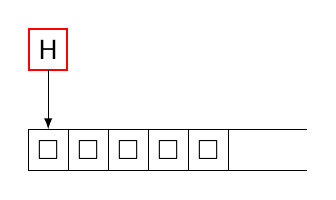
\begin{tikzpicture}[every node/.style={block},
  block/.style={minimum height=1.5em,outer sep=0pt,draw,rectangle,node distance=0pt}]


        \node (A) {$\Box$};
        \node (B) [right = of A] {$\Box$};
        \node (C) [right = of B] {$\Box$};
        \node (D) [right = of C] {$\Box$};
        \node (E) [right = of D] {$\Box$};

        \node (F) [above = 0.75cm of A,draw=red,thick] {\textsf H};
        \draw[-latex] (F) -- (A);

        \draw (E.north east) -- ++(1cm,0) (E.south east) -- ++ (1cm,0);
      \end{tikzpicture}

\end{center}


\underline{Step 3:}

\textbf{Input tape:}
\begin{center}

  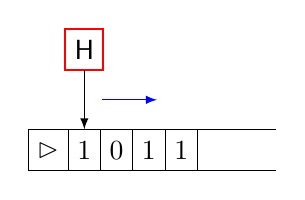
\begin{tikzpicture}[every node/.style={block},
  block/.style={minimum height=1.5em,outer sep=0pt,draw,rectangle,node distance=0pt}]


        \node (A) {$\rhd$};
        \node (B) [right = of A] {1};
        \node (C) [right = of B] {0};
        \node (D) [right = of C] {1};
        \node (E) [right = of D] {1};

        \node (F) [above = 0.75cm of B,draw=red,thick] {\textsf H};
        \draw[-latex] (F) -- (B);

        \draw[-latex,blue] ($(F.east)!0.5!(B.east)$) -- ++(7mm,0);

        \draw (E.north east) -- ++(1cm,0) (E.south east) -- ++ (1cm,0);
      \end{tikzpicture}

\end{center}

\textbf{Work tape:}
\begin{center}

  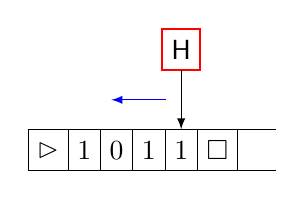
\begin{tikzpicture}[every node/.style={block},
  block/.style={minimum height=1.5em,outer sep=0pt,draw,rectangle,node distance=0pt}]



        \node (A) {$\rhd$};
        \node (B) [right = of A] {1};
        \node (C) [right = of B] {0};
        \node (D) [right = of C] {1};
        \node (E) [right = of D] {1};
        \node (G) [right = of E] {$\Box$};

        \node (F) [above = 0.75cm of E,draw=red,thick] {\textsf H};
        \draw[-latex] (F) -- (E);

        \draw[<-, -latex,blue] ($(C.east)!0.5!(F.east)$) -- ++(-7mm,0);


        \draw (E.north east) -- ++(1cm,0) (E.south east) -- ++ (1cm,0);
      \end{tikzpicture}

\end{center}

\textbf{Output tape:}
\begin{center}

  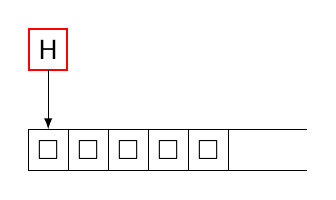
\begin{tikzpicture}[every node/.style={block},
  block/.style={minimum height=1.5em,outer sep=0pt,draw,rectangle,node distance=0pt}]


        \node (A) {$\Box$};
        \node (B) [right = of A] {$\Box$};
        \node (C) [right = of B] {$\Box$};
        \node (D) [right = of C] {$\Box$};
        \node (E) [right = of D] {$\Box$};

        \node (F) [above = 0.75cm of A,draw=red,thick] {\textsf H};
        \draw[-latex] (F) -- (A);

        \draw (E.north east) -- ++(1cm,0) (E.south east) -- ++ (1cm,0);
      \end{tikzpicture}

\end{center}

\textbf{Input tape:}
\begin{center}

  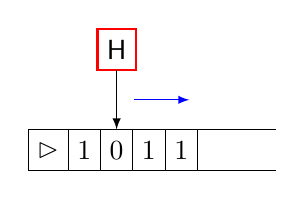
\begin{tikzpicture}[every node/.style={block},
  block/.style={minimum height=1.5em,outer sep=0pt,draw,rectangle,node distance=0pt}]


        \node (A) {$\rhd$};
        \node (B) [right = of A] {1};
        \node (C) [right = of B] {0};
        \node (D) [right = of C] {1};
        \node (E) [right = of D] {1};

        \node (F) [above = 0.75cm of C,draw=red,thick] {\textsf H};
        \draw[-latex] (F) -- (C);

        \draw[-latex,blue] ($(F.east)!0.5!(C.east)$) -- ++(7mm,0);

        \draw (E.north east) -- ++(1cm,0) (E.south east) -- ++ (1cm,0);
      \end{tikzpicture}

\end{center}

\textbf{Work tape:}
\begin{center}

  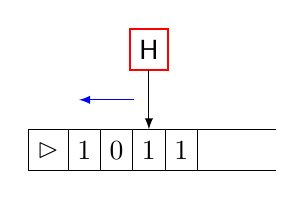
\begin{tikzpicture}[every node/.style={block},
  block/.style={minimum height=1.5em,outer sep=0pt,draw,rectangle,node distance=0pt}]



        \node (A) {$\rhd$};
        \node (B) [right = of A] {1};
        \node (C) [right = of B] {0};
        \node (D) [right = of C] {1};
        \node (E) [right = of D] {1};

        \node (F) [above = 0.75cm of D,draw=red,thick] {\textsf H};
        \draw[-latex] (F) -- (D);

        \draw[<-, -latex,blue] ($(B.east)!0.5!(F.east)$) -- ++(-7mm,0);


        \draw (E.north east) -- ++(1cm,0) (E.south east) -- ++ (1cm,0);
      \end{tikzpicture}

\end{center}

\textbf{Output tape:}
\begin{center}

  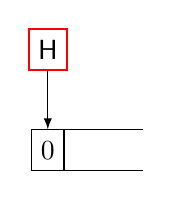
\begin{tikzpicture}[every node/.style={block},
  block/.style={minimum height=1.5em,outer sep=0pt,draw,rectangle,node distance=0pt}]


        \node (A) {$0$};

        \node (F) [above = 0.75cm of A,draw=red,thick] {\textsf H};
        \draw[-latex] (F) -- (A);

        \draw (A.north east) -- ++(1cm,0) (A.south east) -- ++ (1cm,0);
      \end{tikzpicture}

    \end{center}
    \textbf{Note: the formal definition may require a $\rhd$ at the beginning of the ouput tape, the procedure would be adjusted accordingly}

    \subsection{Data representation}

    In many real-world problems our input data does not take the innately take the form of a bitstring, when working with Turing machines, it must be encoded as a bitstring. Not all data can be encoded as bitstrings but many can. An example of data that cannot is any member of the set of Real numbers $\mathbb{R}$.

    Knowing this, we can answer a common question: ``\textit{why don't} we consider Turing machines with more than 1 input? '' the answer: We can simply encode a list of bitstrings as a single bitstring!


\end{document}

